\subsection{Remarkable results in research literature}
Tarjan's algorithm is difficult to parallelize because it is based on DFS graph traversal. For a long time, many researchers believed that no parallel DFS algorithms existed \cite{history-of-parallel-dfs-algorithms}. In the literature, some algorithm for parallelizing DFS were developed, but those algorithms suffer from strong constraints. For example, Reif proposed a parallel algorithm for lexicographical DFS \cite{reif}. Others such as Aggarwal and Anderson, have described algorithms for performing DFS on both undirected and directed graphs \cite{Aggarwal}, but the algorithm is randomized and it requires $n^{2376}$ processors. Other attempts require further restrictions to the graphs under question; for example, Chaudhuri and Hagerup proposed a solution that only works for acyclic and planar graphs. 

\begin{figure}
  \begin{center}
    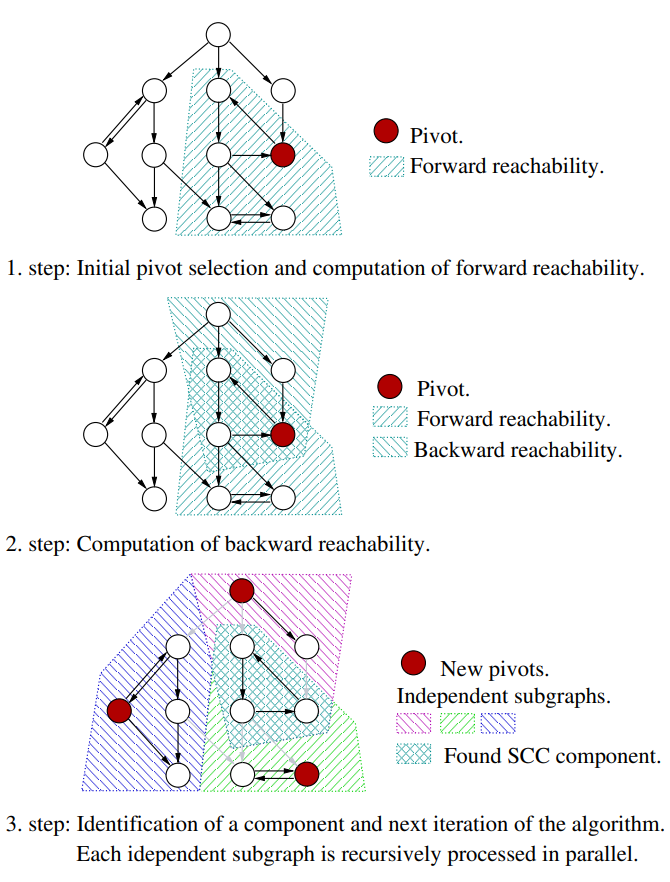
\includegraphics[scale=0.5]{img/fb-algorithm.png}
  \end{center}
  \caption{Key steps of the Forward-Backward Algorithm}
  \label{img:fb-algorithm}
\end{figure}

The most popular algorithms for parallelizing the SCC search in CUDA are the Forward-Backward algorithm (illustrated in Fig. \ref{img:fb-algorithm}), the Coloring algorithm and the OBF algorithm \cite{barnat_bauch_brim_ceka_2011} \cite{usermanual:cuda-sccs}. All of these algorithm are based on BFS traversal because it is much easier to parallelize compared to DFS. Implementing those algorithms in CUDA wouldn't meet the goal of parallelizeing Tarjan's algorithm which is based on DFS. For these reasons, we decided to take a completely different approach: we preprocess the graph to delete trivial SCCs and execute Tarjan's algorithm on the reduced graph. The idea is that, when the number trivial SCCs is substantial, Tarjan's algorithm would benefit from not having to process these nodes. We parallelized the graph preprocesing with CUDA.

\subsection{Graph preprocessing: trivial SCCs deletion}
\label{alg:graph_preprocessing}
The goal of graph preprocessing is to find and mark nodes belonging to trivial SCCs. A trivial SCC is an SCC composed of a single vertex. In other words, we are looking for vertices of the graph that have no immediate predecessors (in the case of leading components) or immediate successors (in the case of terminal components) in the graph. Such vertices may be iteratively removed from the subgraph as trivial SCCs. Futhermore, we also delete SCCs made of a single vertex with a self-loop. The result of the procedure is a bitmask of $|V|$ bits indicating which of the vertices have been eliminated.

\subsection{A CUDA-friendly graph representation}
\label{rep:cuda_graph}
In our sequential implementation of Tarjan's algorithm, discussed in \ref{alg:sequential}, we used the adjacency maps to represent the graphs. This representation is not CUDA-friendly because it is a linked data structure. In order to process the graph with CUDA, we defined the \verb|cuda_graph| struct: we encode the graph as the adjacency list that is represented as two one-dimensional arrays. One array stores the target vertices of edges sorted according to source vertex (\verb|adj_lists|). The second array keeps an index to the first array for each vertex: the index points to the first edge emanating from the vertex (\verb|adj_list_indexes|). A graphical representation of this data structure is shown in Fig. \ref{img:cuda_graph}.

\begin{figure}
  \begin{center}
    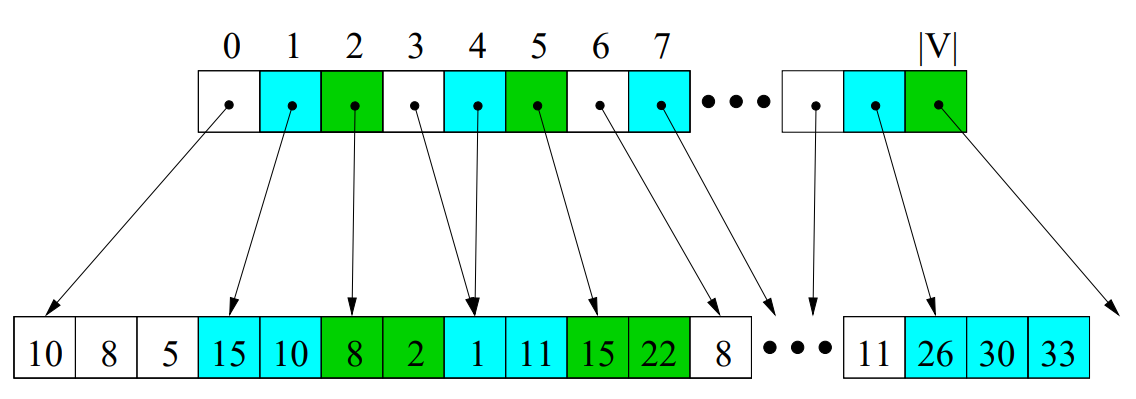
\includegraphics[scale=0.5]{img/cuda_graph.png}
  \end{center}
  \caption{CUDA-friendly graph representation}
  \label{img:cuda_graph}
\end{figure}

\subsection{Steps of the algorithm}
\label{alg:cuda_only}
\noindent The steps of our CUDA-accelerated algorithm are the following:
\begin{enumerate}
  \item Read the graph from the input file as a \verb|cuda_graph| (represented as seen above)
  \item Load the graph on the global memory of the device
  \item Execute a CUDA kernel to mark the nodes to be deleted on a bitmask (as described in \ref{alg:graph_preprocessing})
  \item Move the bitmask from the device to the host
  \item Convert the \verb|cuda_graph| in a \verb|graph| (represented as seen in \ref{alg:sequential}), ignoring the nodes flagged in the bitmask
  \item Execute the sequential version of Tarjan's algorithm on the reduced \verb|graph|
\end{enumerate}
